\section{Теоритические сведения}
\subsection{Дифракция}
Дифракцией называются отклонения в распространении волн от законов геометрической оптики.

Основными параметрами, определяющими характер дифракционных явлений, является длина волны $\lambda$, размер отверстия $b$ и расстояние до плоскости наблюдения $z$. Характер дифоракции определяется волновым параметром

\[
    p = \frac{\sqrt{\lambda z}}{b}
\]

При $p \ll 1$ выполняются законы геометрической оптики, при $p\approx 1$ происзодит дифракция Френеля, $p\gg 1$~--- дифракция Фраунгофера.

\subsection{Принцип Гюйгенса-Френеля}
\begin{figure}[ht!]
    \center{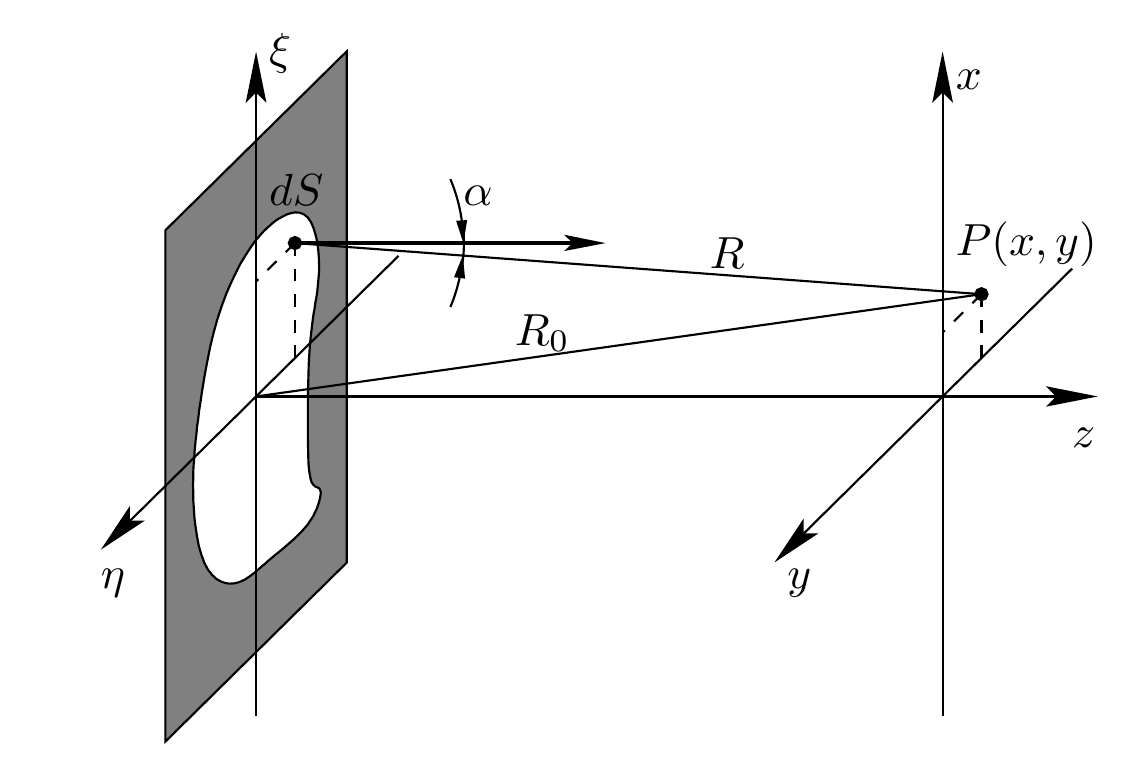
\includegraphics[width=0.8\linewidth]{../img/gufr.png}}
\end{figure}

Пусть волна света, созданная источниками, расположенными в области $z < 0$, достигла плоскости $z=0$. Световое поле в этой плоскости нам известно. Пусть его комплексная амплитуда есть
\[
    f_{0}(x, y) = a_{0}(x, y)e^{i \varphi_{0}(x, y)}
\]
где функции $a_{0}(x, y)$ и $ \varphi_{0}(x, y)$ описывают распределение амплитуд и фаз колебаний в плоскости $z=0$.

Согласно принципу Гюйгенса, каждую точку $( \xi, \eta)$ плоскости $z = 0$, куда пришла волна, можно рассматривать  как источник вторичной волны. То есть можно представить себе, что волна возбуждает колебания некоторого фиктивного источника (осциллятора), который и переизлучает вторичную волну. Частота $ \omega$ этой переизлучённой волны совпадает с частотой исходной монохроматической волны. Френель дополнил принцип Гюйгенса, предложив рассматривать световое колебание в любой точке наблюдения в области $z > 0$ как результат интерференции этих вторичных волн.

Предполагается, что амплитуда излучения вторичного источника пропорциональна амплитуде $a_{0}(\xi, \eta)$  колебания, созданного реальной волной, пришедшей к площадке $ds$. Фаза колебания также задаётся фазой $ \varphi( \xi, \eta)$ пришедшей к элементу $ds$ волны.

Далее предполагается, что маленькая площадка $ds$ переизлучает, подобно точечному источнику, сферическую волну, т. е. для вычисления вклада, который даёт эта площадка в суммарное колебание в точке наблюдения $P$,  нужно учесть ослабление амплитуды и набег фазы $e^{ikR}/R$. Наконец, предполагается, что амплитуда колебания пропорциональна видимой из точки наблюдения площади элемента $ds$, т.е. пропорциональна $ds\cos\alpha$. Таким образом, вклад элемента $ds$ пропорционален величине
\[
    f_{0}(\xi, \eta)\frac{e^{ikR}}{R}\cos\alpha\cdot d\xi d\eta
\]
Полное световое колебание $g(x, y)$ есть результат интерференции всех вторичных волн, посылаемых всеми площадками $ds$, расположенными в области отверстия:
\[
    g(x, y) = \frac{1}{i\lambda}\iint_{S} f_{0}(\xi, \eta)\frac{e^{ikR}}{R}\cos\alpha d\xi d\eta
\]

При условии, что размер препятствия мал по сравнению с расстоянием $R_{0}$ до точки наблюдения, амплитудный множитель $\frac{1}{R}$,  учитывающий уменьшение амплитуды в сферической волне по мере удаления от вторичного источника $ds$, можно заменить постоянной величиной $\frac{1}{R_{0}}$. Множитель наклона $\cos\alpha$ также считаем приблизительно одинаковым (и равным единице) для всех вторичных источников, расположенных в области отверстия. Тогда в этом приближении принцип Гюйгенса—Френеля приобретает следующий вид:
\[
    g(x, y) = \frac{1}{i\lambda R_{0}} \iint f_{0}(\xi, \eta)e^{ikR} d\xi d\eta
\]
\[
    R \approx z + \frac{\left(x - \xi\right)^{2}}{2z} + \frac{\left(y - \eta\right)^{2}}{2z}
\]

Тогда
\[
    g(x, y) = \frac{e^{ikz}}{i \lambda z}\iint f_{0}(\xi, \eta)e^{i\frac{k}{2z}\left(\left(x-\xi\right)^{2} + \left(y - \eta\right)^{2}\right)} d\xi d\eta
\]
Если отверстиеосвещается плоской волной, то $f_{0}(\xi, \eta) = A_{0}$.

\subsection{Дифракция Френеля}

Рассмотрим дифракцию плоской волны амплитуды $A_{0}$ на непрозрачном экране, отверстие в котором имеет вид длинной щели, вытянутой вдоль оси $\eta$. Верхний край щели совпадает с прямой $\xi = b_{1}$, а нижний~--- с $\xi = b_{2}$. Нас интересует световое колебание в точке $P$, расположенной на расстоянии $z$за щелью на оси $z$. Интегрирование по $\eta$ в бесконечных пределах даёт константу, не представляющую интерес. Тогда с точностью до несущественного постоянного множителя получаем
\[
    g = A_{0} \int_{b_{1}}^{b_{2}} e^{\frac{ik}{2z}\xi^{2}}d\xi
\]

Для расчёта светового поля воспользуемся методом векторных диаграмм. Разбив щель на узкие полоски $d\xi$, параллельные краям щели,изобразим колебание, созданное полоской в точке наблюдения $P$, в виде вектора, длина которого равна $d\xi$, а угол наклона $ \varphi = \frac{k}{2z}\xi^{2}$. В частности, вклад полоски вторичныхисточников, лежащих на оси $\eta$, изображается горизонтальным вектором.

Разность фаз $d\varphi$  колебаний от полосок на расстояниях $\xi$ и $\xi + d\xi$:
\[
    d\varphi = \frac{k}{z}\xi d\xi
\]
Поэтому угол между двумя соседними векторами на диаграмме не сохраняется неизменным. По мере удаления от центра угол начинает быстро нарастать~--- цепочка векторов быстро скручивается.

\begin{figure}[ht!]
    \center{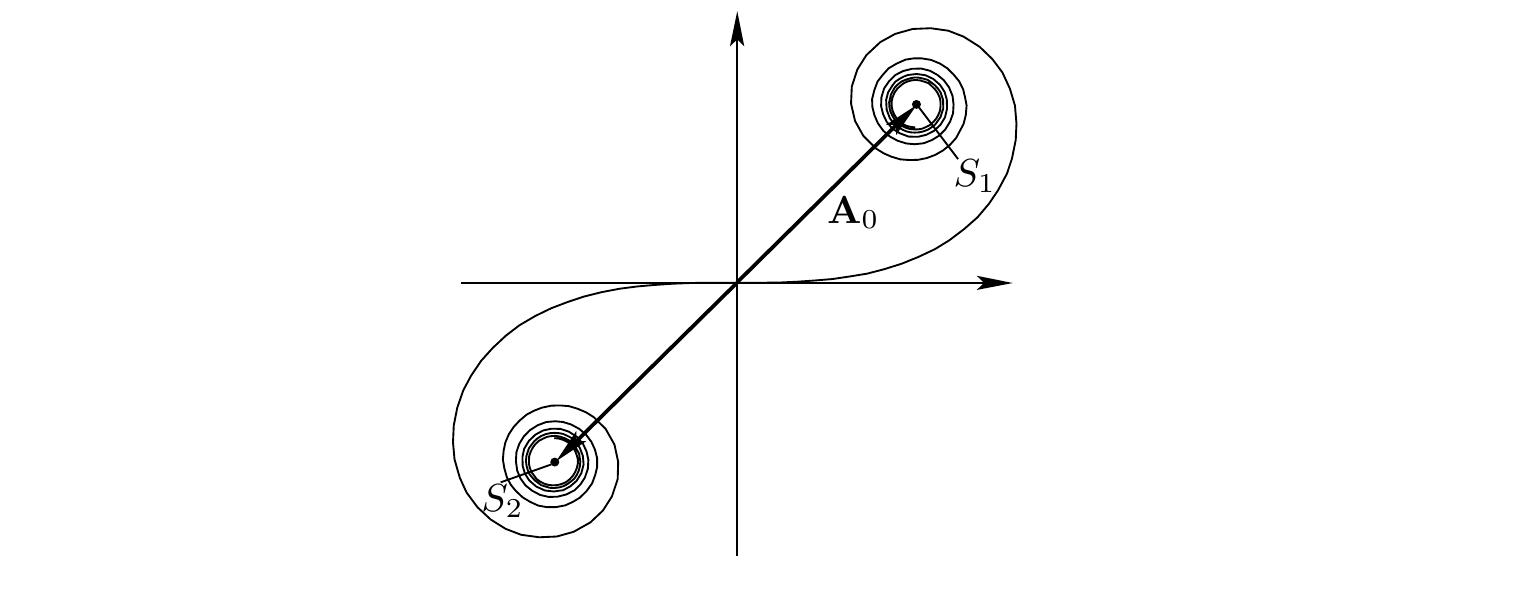
\includegraphics[width=0.8\linewidth]{../img/korney.png}}
\end{figure}

Диаграмму можно разделить на части, вклад каждой из которых в сдиг фаз будет $\pi$. Каждой такой части соответствует своя зона Шустера~--- прямоугольная часть щели. Т.к. сдвиг фаз между соседними зонами Шустера $\pi$, ширина зоны $m$ равна
\[
    \frac{k}{2z}\left(r_{m} / 2\right)^{2} = \pi m
\]
\[
    r_{m} = 2 \sqrt{2\pi m z / k} = 2 \sqrt{ \lambda z}
\]

\subsection{Дифракция Фраунгофера}
Рассмотрим дифракцию на отверстии в плоском экране, находящемся в плоскости $z = 0$. Пусть точка наблюдения имеет координаты $P(x, y, z)$. Расстояние $R$  от площадки $ds$ в точке экрана $(\xi, \eta)$ до точки $P$ равно
\[
    R = sqrt{z^{2} + \left(x - \xi\right)^{2} + \left(y - \eta\right)^{2}}\approx R_{0} - \frac{x\xi + y\eta}{R_{0}} + \frac{\xi^{2} + \eta^{2}}{2R_{0}}
\]
$R_{0} = \sqrt{x^{2} + y^{2} + z^{2}}$~--- расстояние от начала координат $O$ до точки наблюдения.
\[
    \xi^{2} + \eta^{2} \le b^{2} \ll \lambda R_{0}
\]
Тогда последним слагаемым в $R$ можно пренебречь и
\[
    R\approx R_{0} -\frac{x\xi}{R_{0}} - \frac{y\eta}{R_{0}}
\]

Тогда принцип Гюйгенса-Френеля запишется в виде
\[
    g(x, y) = \frac{e^{ikR_{0}}}{i\lambda R_{0}}\iint f_{0}(\xi, \eta)e^{-i\left(\frac{kx}{R_{0}}\xi + \frac{ky}{R_{0}}\eta\right)} d\xi d\eta
\]
В одномерном случае
\[
    g(x) ~ \int_{-\infty}^{+\infty} f_{0}(\xi)e^{-\frac{ikx\xi}{R_{0}}}d\xi
\]
$u = \frac{kx}{R_{0}}$, а картина дифракции Фраунгофера представляет собой преобразование Фурье граничного поля $f_{0}(\xi)$. 

\begin{figure}[ht!]
    \center{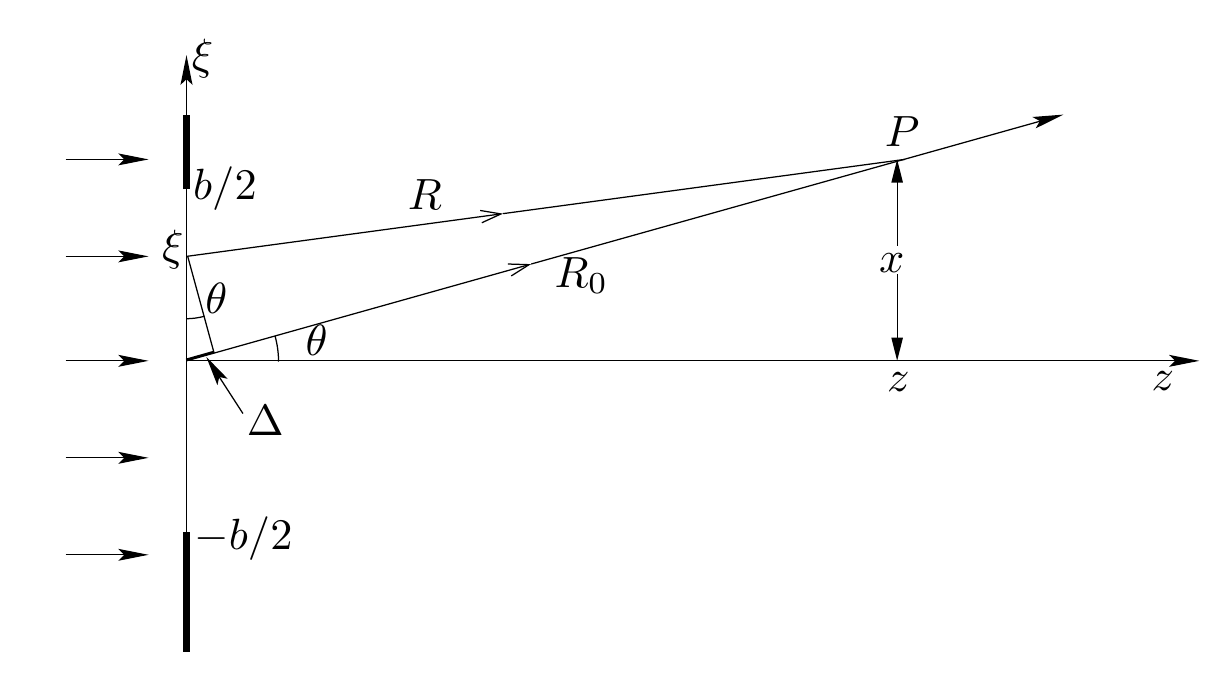
\includegraphics[width=0.8\linewidth]{../img/frau.png}}
\end{figure}

Определим разность хода волн $\Delta$,  приходящих к удалённой точке наблюдения от двух вторичных источников, один из которых находится в точке с координатой $\xi$, а второй — в точке $\xi = 0$. Удалённость точки $P$  позволяет считать направления волн, идущих из этих точек практически параллельными, следовательно, разность их хода равна
\[
    \Delta = \xi \sin \theta
\]
Соответственно разность фаз колебаний равна $ \varphi = -k\xi \sin \theta$, где $ \theta$~--- направление на удалённую точку наблюдения, имеющую координату $x$:
\[
    k\sin \theta = \frac{kx}{R_{0}} = u
\]

Таким образом
\[
    g(u) ~ \int_{-\infty}^{+\infty} f_{0}(\xi)e^{-ik\sin \theta \xi} d\xi
\]

Эта формула~--- полный аналог преобразования Фурье для $f_{0}(t)$
\[
    C(\omega) = \int f_{0}(t)e^{-i\omega t} dt
\]

Эта аналлогия позволяет назвать величину $u=k\sin \theta$ пространственной частотой.

Распределение $I(\theta) ~ g(\theta)$ называется диаграммой направленности.

\subsection{Дифракция Фраунгофера на щели}
Пусть щель шириной $b$ освещается слева плоской нормально падающей волной. Граничное поле $f_{0}(x)$, возникающее в плоскости $z = 0$, примыкающей к непрозрачному экрану со щелью справа, имеет вид прямоугольного выступа шириной $b$. Тогда 
\[
    g(\theta) ~ \int_{-b/2}^{b/2} e^{ikx\sin \theta}dx ~ \frac{\frac{kb}{2}\sin \theta}{\frac{kb}{2}\sin \theta}
\]
\begin{figure}[ht!]
    \center{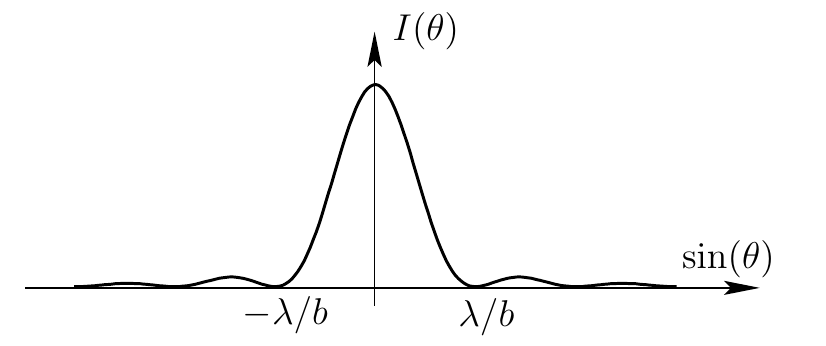
\includegraphics[width=0.8\linewidth]{../img/frau1.png}}
\end{figure}


Почти вся интенсивность $I(\theta) ~ g(\theta)^{2}$ сосредоточена в области
\[
    \left|\sin \theta \right| \le \frac{ \lambda}{b}
\]

\subsection{Дифракция Фраунгофера на двух щелях}
Рядом со щелью, дифракцию на которой мы рассмотрели выше, расположим параллельно ещё одну щель на расстоянии $d$ от первой.

Расстояние от второй щели до точки наблюдения на величину $ \Delta = d\sin\theta$  меньше расстояния между первой щелью и точкой наблюдения. Соответствующая фаза колебания отличается на величину
\[
    \alpha = -k \Delta = -kd \sin \theta
\]
Поэтому колебательный процесс, созданный второй щелью в точке наблюдения, описывается функцией $g( \theta)e^{i \alpha}$.  Волны, посылаемые в точку наблюдения двумя щелями, интерферируют. Амплитуда суммарного колебательного процесса в точке наблюдения есть $g( \theta) + g( \theta)e^{i \alpha}$.

Картина интенсивности 
\[
    I( \theta) ~ \left| g( \theta) \right|^{2} \left(1 + \cos \left(kd \sin \theta\right)\right)^{2}
\]

\begin{figure}[ht!]
    \center{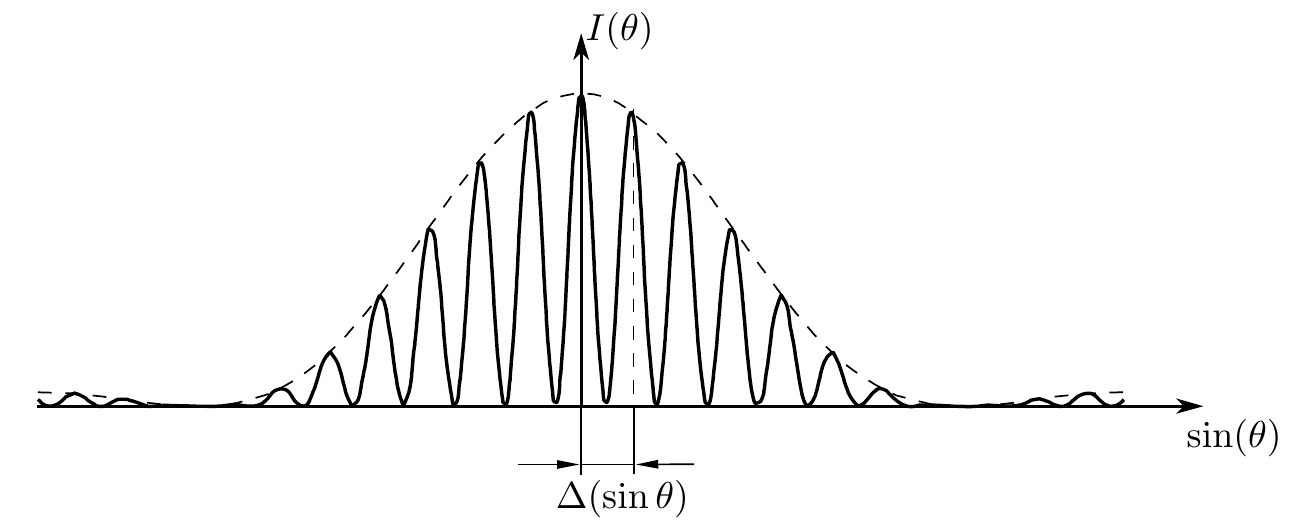
\includegraphics[width=0.8\linewidth]{../img/frau2.png}}
\end{figure}

\subsection{Пространственная когерентность}
\begin{figure}[ht!]
    \center{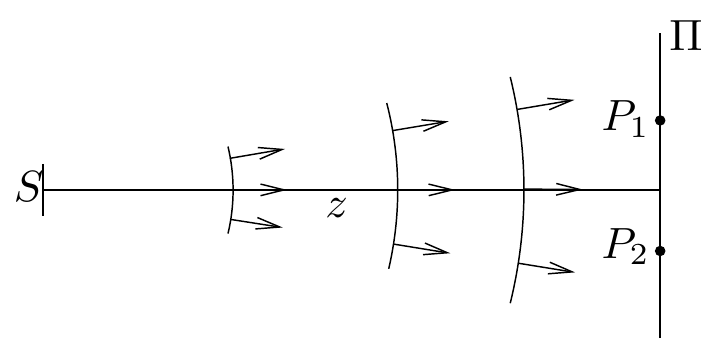
\includegraphics[width=0.8\linewidth]{../img/pkog1.png}}
\end{figure}

Пусть источником светового поля $E(\vec{r}, t)$ в плоскости наблюдения П является протяжённый квазимонохроматический источник S, находящийся на расстоянии $z$. Колебания поля в точках $P_{1}$ и $P_{2}$ плоскости наблюдения запишем, в комплексной форме
\[
    V_{1}(t) = A_{1}(\vec{r}_{1}, t)e^{iwt},\;\; V_{2}(t) = A_{2}(\vec{r}_{2}, t)e^{iwt}
\]
Рассмотрим вопрос о когерентности колебаний $V_{1}(t)$ и $V_{2}(t)$.  Каждый из колебательных процессов характеризуется временем когерентности $\tau_{0}$, т.е. в течение времени $\tau \ll \tau_{0}$ амплитуды $a_{i}(t)$ и фазы колебаний $\varphi_{i}(t)$ сохраняются почти неизменными. По прошествии времени $\tau_{0}$ амплитуды и фазы колебаний принимают новые значения, которые некоррелированы со своими прежними значениями. Если при этом разности фаз сохраняются, то колебания будут когерентными.

Рассмотрение колебаний в различных точках пространства позволяет ввести понятие пространственной когерентности. Количественной мерой пространственной когерентности является функция пространственной когерентности:
\[
    \Gamma_{12} = \overline{V_{1}(t)V_{2}^{*}(t)} = \overline{A_{1}(t)A_{2}^{*}(t)} 
\]
которая зависит от расстояния между точками наблюдения. Нормированная функция
\[
    \gamma_{12} = \frac{\overline{V_{1}(t)V_{2}^{*}(t)}}{\sqrt{I_{1}I_{2}}}
\]
называется степенью пространственной когерентности.

Вопрос о пространственной когерентности возникает, если источникявляется протяжённым, и разные его участки $ds$излучают некогерентно. Действительно, излучение разных участков~--- это излучение разных совокупностей атомов, моменты возникновения излучаемых ими цугов не связаны между собой, поэтому разность фаз излучаемых ими волн изменяется за время регистрации $\Delta t \gg \tau_{0}$ множество раз, принимая с равной вероятностью любое значение в интервале $\left[0,2\pi]\right]$

Найдём колебания поля, созданного протяжённым квазимонохроматическим источником S в точках $P_{1}(x_{1})$ и $P_{2}(x_{2})$ плоскости наблюдения, находящейся на расстоянии $z$ от источника~--- излучающего отрезка ширины $b$, расстояние между точками $P_{1}$ и $P_{2}$ равно $\rho = |x_{1} - x_{2}|$. Колебания в каждой из точек $P_{1}$  и $P_{2}$~--- это сумма колебаний, созданных всеми малыми отрезками $\Delta\xi$  источника. Амплитуда $a_{i} = a(\xi_{i})$ колебаний излучающей площадки $\Delta\xi_{i}$, имеющей координату $\xi_{i}$, и её фаза $\varphi_{i} = \varphi(\xi_{i})$ сохраняются неизменными в течение времени, малом по сравнению со временем когерентности $\tau_{0}$. При распространении волны от площадки $\Delta\xi_{i}$ до точек $P_{1}$ и $P_{2}$ возникает набег фазы $kr_{1i}$ и $kr_{2i}$  соответственно. Поэтому суммарное колебание в точках $P_{1}$ и $P_{2}$ можно записать в виде
\[
    A_{1} = \sum_{i}a_{i}e^{i\varphi}\frac{e^{ikr_{1i}}}{r_{1i}}\;\;A_{2} = \sum_{i}a_{i}e^{i\varphi}\frac{e^{ikr_{2i}}}{r_{2i}}
\]

$A_{1}$ и $A_{2}$~--- комплексные амплитуды.

\[
    A_{1}A_{2}^{*} = \sum_{i}\sum_{j}a_{i}a_{j}e^{i\left( \varphi_{i} - \varphi_{j}\right)}\frac{e^{ik\left(r_{1i} - r_{2i}\right)}}{r_{1i}r_{2i}}
\]

\begin{figure}[ht!]
    \center{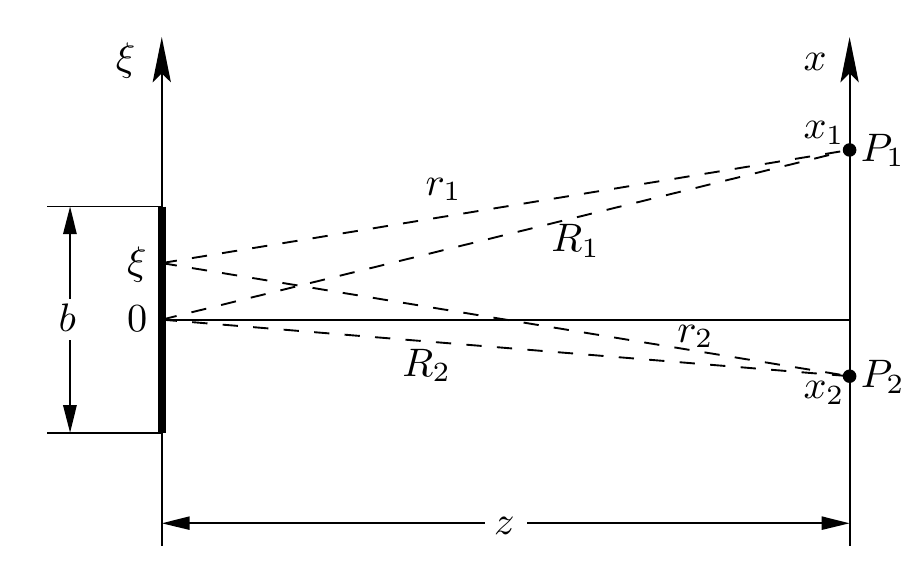
\includegraphics[width=0.8\linewidth]{../img/pkog2.png}}
\end{figure}
При усреднении величины $A_{1}A_{2}^{*}$ за время $\Delta t \gg \tau_{0}$ учтём некогерентность колебаний, созданных разными площадками
\[
    \overline{A_{1}A_{2}^{*}} = \sum_{i}\overline{a_{i}^{2}}\frac{e^{ik\left(r_{1i}-r_{2i}\right)}}{r_{1}r_{2}}
\]

Далее мы учтём, что среднее значение квадрата амплитуды излучающей площадки $\Delta\xi$ равно $\overline{a^{2}\left(\xi\right)} = J(\xi) \Delta\xi$, где $J(\xi)$~---  интенсивность излучения единичной площадки, имеющей координату $\xi$. Примем также, что размеры источника $b$ и расстояние $\rho$ малы по сравнению с $z$.  В этом приближении можно положить
\[
    \frac{1}{r_{1}r_{2}} \approx \frac{1}{R_{1}R_{2}}
\]
 При вычислении фазового множителя $e^{ik\left(r_{1}-r_{2}\right)}$ необходимо учесть дополнительный член в разложении $r_{1},\; r_{2}$ в ряд Тейлора, поскольку ошибки при оценке должны быть малы по сравнению с длиной волны $\lambda$. Тогда
 \[
     r_{1,2} = \sqrt{z^{2} + \left(x_{1,2} - \xi\right)^{2}} \approx z + \frac{\left(x_{1,2} - \xi\right)^{2}}{2z}
 \]
при условии, что отброшенные члены разложения много меньше $\lambda$. Отсюда
\[
    r_{1} - r_{2} \approx \frac{x_{1}^{2} - x^{2}_{2}}{2z} - \frac{\rho\xi}{z}
\]
Тогда
\[
    \Gamma(\rho) = \overline{V_{1}(t)V_{2}^{*}(t)} = \overline{A_{1}(t)A_{2}^{*}(t)} = \frac{e^{ik\rho x/z}}{R_{1}R_{2}}\int J(\xi)e^{-ik\rho\xi / z} d\xi
\]
$x = (x_{1} + x_{2}) / 2$.
\[
    \gamma(\rho) = \frac{\int J(\xi)e^{-ik\rho\xi / z} d\xi}{\int J(\xi)d\xi}
\]
Функция пространственной когерентности $\Gamma(\rho)$ является преобразованием Фурье распределения интенсивности излучения по источнику $J(\xi)$. В роли частоты $\omega$ здесь выступает пространственная частота $\frac{k\rho}{z}$.

Для однородного источника (все точки которого излучают с одинаковой интенсивностью $J_{0}$)

\[
    \gamma(\rho) = \frac{\sin \frac{kb}{2z}\rho}{\frac{kb}{2z}\rho}
\]

Найдём радиус пространственной когерентности $\rho_{0}$~--- максимальное расстояние между точками наблюдения, при котором степень когерентности не обращается в нуль. Его можно оценить по полуширине главного максимума функции $\gamma(\rho)$:
\[
    \rho_{0} = \frac{\lambda z}{b} = \frac{\lambda}{\psi}
\]

Функция $\gamma(\rho)$ описывает постепенное уменьшение степени когерентности от единицы при $\rho = 0$ до нуля по мере увеличения расстояния между точками наблюдения. При $\rho = \rho_{0}$ степень когерентности становится равной нулю. Отметим однако, что наличие боковых лепестков функции $\gamma(\rho)$ означает частичное (незначительное) восстановление степени когерентности колебаний в точках, расстояние между которыми превышает $\rho_{0}$.
